
% Default to the notebook output style

    


% Inherit from the specified cell style.




    
\documentclass[11pt]{article}

    
    

    \usepackage[T1]{fontenc}
    % Nicer default font (+ math font) than Computer Modern for most use cases
    \usepackage{mathpazo}

    % Basic figure setup, for now with no caption control since it's done
    % automatically by Pandoc (which extracts ![](path) syntax from Markdown).
    \usepackage{graphicx}
    % We will generate all images so they have a width \maxwidth. This means
    % that they will get their normal width if they fit onto the page, but
    % are scaled down if they would overflow the margins.
    \makeatletter
    \def\maxwidth{\ifdim\Gin@nat@width>\linewidth\linewidth
    \else\Gin@nat@width\fi}
    \makeatother
    \let\Oldincludegraphics\includegraphics
    % Set max figure width to be 80% of text width, for now hardcoded.
    \renewcommand{\includegraphics}[1]{\Oldincludegraphics[width=.8\maxwidth]{#1}}
    % Ensure that by default, figures have no caption (until we provide a
    % proper Figure object with a Caption API and a way to capture that
    % in the conversion process - todo).
    \usepackage{caption}
    \DeclareCaptionLabelFormat{nolabel}{}
    \captionsetup{labelformat=nolabel}

    \usepackage{adjustbox} % Used to constrain images to a maximum size 
    \usepackage{xcolor} % Allow colors to be defined
    \usepackage{enumerate} % Needed for markdown enumerations to work
    \usepackage{geometry} % Used to adjust the document margins
    \usepackage{amsmath} % Equations
    \usepackage{amssymb} % Equations
    \usepackage{textcomp} % defines textquotesingle
    % Hack from http://tex.stackexchange.com/a/47451/13684:
    \AtBeginDocument{%
        \def\PYZsq{\textquotesingle}% Upright quotes in Pygmentized code
    }
    \usepackage{upquote} % Upright quotes for verbatim code
    \usepackage{eurosym} % defines \euro
    \usepackage[mathletters]{ucs} % Extended unicode (utf-8) support
    \usepackage[utf8x]{inputenc} % Allow utf-8 characters in the tex document
    \usepackage{fancyvrb} % verbatim replacement that allows latex
    \usepackage{grffile} % extends the file name processing of package graphics 
                         % to support a larger range 
    % The hyperref package gives us a pdf with properly built
    % internal navigation ('pdf bookmarks' for the table of contents,
    % internal cross-reference links, web links for URLs, etc.)
    \usepackage{hyperref}
    \usepackage{longtable} % longtable support required by pandoc >1.10
    \usepackage{booktabs}  % table support for pandoc > 1.12.2
    \usepackage[inline]{enumitem} % IRkernel/repr support (it uses the enumerate* environment)
    \usepackage[normalem]{ulem} % ulem is needed to support strikethroughs (\sout)
                                % normalem makes italics be italics, not underlines
    
\usepackage[round]{natbib}
\usepackage{pgf}
\usepackage{tikz}
\usetikzlibrary{positioning}
\usepackage{algorithmic}
\usepackage[ruled, vlined, linesnumbered]{algorithm2e}


    
    
    % Colors for the hyperref package
    \definecolor{urlcolor}{rgb}{0,.145,.698}
    \definecolor{linkcolor}{rgb}{.71,0.21,0.01}
    \definecolor{citecolor}{rgb}{.12,.54,.11}

    % ANSI colors
    \definecolor{ansi-black}{HTML}{3E424D}
    \definecolor{ansi-black-intense}{HTML}{282C36}
    \definecolor{ansi-red}{HTML}{E75C58}
    \definecolor{ansi-red-intense}{HTML}{B22B31}
    \definecolor{ansi-green}{HTML}{00A250}
    \definecolor{ansi-green-intense}{HTML}{007427}
    \definecolor{ansi-yellow}{HTML}{DDB62B}
    \definecolor{ansi-yellow-intense}{HTML}{B27D12}
    \definecolor{ansi-blue}{HTML}{208FFB}
    \definecolor{ansi-blue-intense}{HTML}{0065CA}
    \definecolor{ansi-magenta}{HTML}{D160C4}
    \definecolor{ansi-magenta-intense}{HTML}{A03196}
    \definecolor{ansi-cyan}{HTML}{60C6C8}
    \definecolor{ansi-cyan-intense}{HTML}{258F8F}
    \definecolor{ansi-white}{HTML}{C5C1B4}
    \definecolor{ansi-white-intense}{HTML}{A1A6B2}

    % commands and environments needed by pandoc snippets
    % extracted from the output of `pandoc -s`
    \providecommand{\tightlist}{%
      \setlength{\itemsep}{0pt}\setlength{\parskip}{0pt}}
    \DefineVerbatimEnvironment{Highlighting}{Verbatim}{commandchars=\\\{\}}
    % Add ',fontsize=\small' for more characters per line
    \newenvironment{Shaded}{}{}
    \newcommand{\KeywordTok}[1]{\textcolor[rgb]{0.00,0.44,0.13}{\textbf{{#1}}}}
    \newcommand{\DataTypeTok}[1]{\textcolor[rgb]{0.56,0.13,0.00}{{#1}}}
    \newcommand{\DecValTok}[1]{\textcolor[rgb]{0.25,0.63,0.44}{{#1}}}
    \newcommand{\BaseNTok}[1]{\textcolor[rgb]{0.25,0.63,0.44}{{#1}}}
    \newcommand{\FloatTok}[1]{\textcolor[rgb]{0.25,0.63,0.44}{{#1}}}
    \newcommand{\CharTok}[1]{\textcolor[rgb]{0.25,0.44,0.63}{{#1}}}
    \newcommand{\StringTok}[1]{\textcolor[rgb]{0.25,0.44,0.63}{{#1}}}
    \newcommand{\CommentTok}[1]{\textcolor[rgb]{0.38,0.63,0.69}{\textit{{#1}}}}
    \newcommand{\OtherTok}[1]{\textcolor[rgb]{0.00,0.44,0.13}{{#1}}}
    \newcommand{\AlertTok}[1]{\textcolor[rgb]{1.00,0.00,0.00}{\textbf{{#1}}}}
    \newcommand{\FunctionTok}[1]{\textcolor[rgb]{0.02,0.16,0.49}{{#1}}}
    \newcommand{\RegionMarkerTok}[1]{{#1}}
    \newcommand{\ErrorTok}[1]{\textcolor[rgb]{1.00,0.00,0.00}{\textbf{{#1}}}}
    \newcommand{\NormalTok}[1]{{#1}}
    
    % Additional commands for more recent versions of Pandoc
    \newcommand{\ConstantTok}[1]{\textcolor[rgb]{0.53,0.00,0.00}{{#1}}}
    \newcommand{\SpecialCharTok}[1]{\textcolor[rgb]{0.25,0.44,0.63}{{#1}}}
    \newcommand{\VerbatimStringTok}[1]{\textcolor[rgb]{0.25,0.44,0.63}{{#1}}}
    \newcommand{\SpecialStringTok}[1]{\textcolor[rgb]{0.73,0.40,0.53}{{#1}}}
    \newcommand{\ImportTok}[1]{{#1}}
    \newcommand{\DocumentationTok}[1]{\textcolor[rgb]{0.73,0.13,0.13}{\textit{{#1}}}}
    \newcommand{\AnnotationTok}[1]{\textcolor[rgb]{0.38,0.63,0.69}{\textbf{\textit{{#1}}}}}
    \newcommand{\CommentVarTok}[1]{\textcolor[rgb]{0.38,0.63,0.69}{\textbf{\textit{{#1}}}}}
    \newcommand{\VariableTok}[1]{\textcolor[rgb]{0.10,0.09,0.49}{{#1}}}
    \newcommand{\ControlFlowTok}[1]{\textcolor[rgb]{0.00,0.44,0.13}{\textbf{{#1}}}}
    \newcommand{\OperatorTok}[1]{\textcolor[rgb]{0.40,0.40,0.40}{{#1}}}
    \newcommand{\BuiltInTok}[1]{{#1}}
    \newcommand{\ExtensionTok}[1]{{#1}}
    \newcommand{\PreprocessorTok}[1]{\textcolor[rgb]{0.74,0.48,0.00}{{#1}}}
    \newcommand{\AttributeTok}[1]{\textcolor[rgb]{0.49,0.56,0.16}{{#1}}}
    \newcommand{\InformationTok}[1]{\textcolor[rgb]{0.38,0.63,0.69}{\textbf{\textit{{#1}}}}}
    \newcommand{\WarningTok}[1]{\textcolor[rgb]{0.38,0.63,0.69}{\textbf{\textit{{#1}}}}}
    
    
    % Define a nice break command that doesn't care if a line doesn't already
    % exist.
    \def\br{\hspace*{\fill} \\* }
    % Math Jax compatability definitions
    \def\gt{>}
    \def\lt{<}
    % Document parameters
    
\title{Inverse Probability of Treatment Weighting Under Violations of Positivity}

    
    
\author{Tomas D. Morley}

    

    % Pygments definitions
    
\makeatletter
\def\PY@reset{\let\PY@it=\relax \let\PY@bf=\relax%
    \let\PY@ul=\relax \let\PY@tc=\relax%
    \let\PY@bc=\relax \let\PY@ff=\relax}
\def\PY@tok#1{\csname PY@tok@#1\endcsname}
\def\PY@toks#1+{\ifx\relax#1\empty\else%
    \PY@tok{#1}\expandafter\PY@toks\fi}
\def\PY@do#1{\PY@bc{\PY@tc{\PY@ul{%
    \PY@it{\PY@bf{\PY@ff{#1}}}}}}}
\def\PY#1#2{\PY@reset\PY@toks#1+\relax+\PY@do{#2}}

\expandafter\def\csname PY@tok@w\endcsname{\def\PY@tc##1{\textcolor[rgb]{0.73,0.73,0.73}{##1}}}
\expandafter\def\csname PY@tok@c\endcsname{\let\PY@it=\textit\def\PY@tc##1{\textcolor[rgb]{0.25,0.50,0.50}{##1}}}
\expandafter\def\csname PY@tok@cp\endcsname{\def\PY@tc##1{\textcolor[rgb]{0.74,0.48,0.00}{##1}}}
\expandafter\def\csname PY@tok@k\endcsname{\let\PY@bf=\textbf\def\PY@tc##1{\textcolor[rgb]{0.00,0.50,0.00}{##1}}}
\expandafter\def\csname PY@tok@kp\endcsname{\def\PY@tc##1{\textcolor[rgb]{0.00,0.50,0.00}{##1}}}
\expandafter\def\csname PY@tok@kt\endcsname{\def\PY@tc##1{\textcolor[rgb]{0.69,0.00,0.25}{##1}}}
\expandafter\def\csname PY@tok@o\endcsname{\def\PY@tc##1{\textcolor[rgb]{0.40,0.40,0.40}{##1}}}
\expandafter\def\csname PY@tok@ow\endcsname{\let\PY@bf=\textbf\def\PY@tc##1{\textcolor[rgb]{0.67,0.13,1.00}{##1}}}
\expandafter\def\csname PY@tok@nb\endcsname{\def\PY@tc##1{\textcolor[rgb]{0.00,0.50,0.00}{##1}}}
\expandafter\def\csname PY@tok@nf\endcsname{\def\PY@tc##1{\textcolor[rgb]{0.00,0.00,1.00}{##1}}}
\expandafter\def\csname PY@tok@nc\endcsname{\let\PY@bf=\textbf\def\PY@tc##1{\textcolor[rgb]{0.00,0.00,1.00}{##1}}}
\expandafter\def\csname PY@tok@nn\endcsname{\let\PY@bf=\textbf\def\PY@tc##1{\textcolor[rgb]{0.00,0.00,1.00}{##1}}}
\expandafter\def\csname PY@tok@ne\endcsname{\let\PY@bf=\textbf\def\PY@tc##1{\textcolor[rgb]{0.82,0.25,0.23}{##1}}}
\expandafter\def\csname PY@tok@nv\endcsname{\def\PY@tc##1{\textcolor[rgb]{0.10,0.09,0.49}{##1}}}
\expandafter\def\csname PY@tok@no\endcsname{\def\PY@tc##1{\textcolor[rgb]{0.53,0.00,0.00}{##1}}}
\expandafter\def\csname PY@tok@nl\endcsname{\def\PY@tc##1{\textcolor[rgb]{0.63,0.63,0.00}{##1}}}
\expandafter\def\csname PY@tok@ni\endcsname{\let\PY@bf=\textbf\def\PY@tc##1{\textcolor[rgb]{0.60,0.60,0.60}{##1}}}
\expandafter\def\csname PY@tok@na\endcsname{\def\PY@tc##1{\textcolor[rgb]{0.49,0.56,0.16}{##1}}}
\expandafter\def\csname PY@tok@nt\endcsname{\let\PY@bf=\textbf\def\PY@tc##1{\textcolor[rgb]{0.00,0.50,0.00}{##1}}}
\expandafter\def\csname PY@tok@nd\endcsname{\def\PY@tc##1{\textcolor[rgb]{0.67,0.13,1.00}{##1}}}
\expandafter\def\csname PY@tok@s\endcsname{\def\PY@tc##1{\textcolor[rgb]{0.73,0.13,0.13}{##1}}}
\expandafter\def\csname PY@tok@sd\endcsname{\let\PY@it=\textit\def\PY@tc##1{\textcolor[rgb]{0.73,0.13,0.13}{##1}}}
\expandafter\def\csname PY@tok@si\endcsname{\let\PY@bf=\textbf\def\PY@tc##1{\textcolor[rgb]{0.73,0.40,0.53}{##1}}}
\expandafter\def\csname PY@tok@se\endcsname{\let\PY@bf=\textbf\def\PY@tc##1{\textcolor[rgb]{0.73,0.40,0.13}{##1}}}
\expandafter\def\csname PY@tok@sr\endcsname{\def\PY@tc##1{\textcolor[rgb]{0.73,0.40,0.53}{##1}}}
\expandafter\def\csname PY@tok@ss\endcsname{\def\PY@tc##1{\textcolor[rgb]{0.10,0.09,0.49}{##1}}}
\expandafter\def\csname PY@tok@sx\endcsname{\def\PY@tc##1{\textcolor[rgb]{0.00,0.50,0.00}{##1}}}
\expandafter\def\csname PY@tok@m\endcsname{\def\PY@tc##1{\textcolor[rgb]{0.40,0.40,0.40}{##1}}}
\expandafter\def\csname PY@tok@gh\endcsname{\let\PY@bf=\textbf\def\PY@tc##1{\textcolor[rgb]{0.00,0.00,0.50}{##1}}}
\expandafter\def\csname PY@tok@gu\endcsname{\let\PY@bf=\textbf\def\PY@tc##1{\textcolor[rgb]{0.50,0.00,0.50}{##1}}}
\expandafter\def\csname PY@tok@gd\endcsname{\def\PY@tc##1{\textcolor[rgb]{0.63,0.00,0.00}{##1}}}
\expandafter\def\csname PY@tok@gi\endcsname{\def\PY@tc##1{\textcolor[rgb]{0.00,0.63,0.00}{##1}}}
\expandafter\def\csname PY@tok@gr\endcsname{\def\PY@tc##1{\textcolor[rgb]{1.00,0.00,0.00}{##1}}}
\expandafter\def\csname PY@tok@ge\endcsname{\let\PY@it=\textit}
\expandafter\def\csname PY@tok@gs\endcsname{\let\PY@bf=\textbf}
\expandafter\def\csname PY@tok@gp\endcsname{\let\PY@bf=\textbf\def\PY@tc##1{\textcolor[rgb]{0.00,0.00,0.50}{##1}}}
\expandafter\def\csname PY@tok@go\endcsname{\def\PY@tc##1{\textcolor[rgb]{0.53,0.53,0.53}{##1}}}
\expandafter\def\csname PY@tok@gt\endcsname{\def\PY@tc##1{\textcolor[rgb]{0.00,0.27,0.87}{##1}}}
\expandafter\def\csname PY@tok@err\endcsname{\def\PY@bc##1{\setlength{\fboxsep}{0pt}\fcolorbox[rgb]{1.00,0.00,0.00}{1,1,1}{\strut ##1}}}
\expandafter\def\csname PY@tok@kc\endcsname{\let\PY@bf=\textbf\def\PY@tc##1{\textcolor[rgb]{0.00,0.50,0.00}{##1}}}
\expandafter\def\csname PY@tok@kd\endcsname{\let\PY@bf=\textbf\def\PY@tc##1{\textcolor[rgb]{0.00,0.50,0.00}{##1}}}
\expandafter\def\csname PY@tok@kn\endcsname{\let\PY@bf=\textbf\def\PY@tc##1{\textcolor[rgb]{0.00,0.50,0.00}{##1}}}
\expandafter\def\csname PY@tok@kr\endcsname{\let\PY@bf=\textbf\def\PY@tc##1{\textcolor[rgb]{0.00,0.50,0.00}{##1}}}
\expandafter\def\csname PY@tok@bp\endcsname{\def\PY@tc##1{\textcolor[rgb]{0.00,0.50,0.00}{##1}}}
\expandafter\def\csname PY@tok@vc\endcsname{\def\PY@tc##1{\textcolor[rgb]{0.10,0.09,0.49}{##1}}}
\expandafter\def\csname PY@tok@vg\endcsname{\def\PY@tc##1{\textcolor[rgb]{0.10,0.09,0.49}{##1}}}
\expandafter\def\csname PY@tok@vi\endcsname{\def\PY@tc##1{\textcolor[rgb]{0.10,0.09,0.49}{##1}}}
\expandafter\def\csname PY@tok@sb\endcsname{\def\PY@tc##1{\textcolor[rgb]{0.73,0.13,0.13}{##1}}}
\expandafter\def\csname PY@tok@sc\endcsname{\def\PY@tc##1{\textcolor[rgb]{0.73,0.13,0.13}{##1}}}
\expandafter\def\csname PY@tok@s2\endcsname{\def\PY@tc##1{\textcolor[rgb]{0.73,0.13,0.13}{##1}}}
\expandafter\def\csname PY@tok@sh\endcsname{\def\PY@tc##1{\textcolor[rgb]{0.73,0.13,0.13}{##1}}}
\expandafter\def\csname PY@tok@s1\endcsname{\def\PY@tc##1{\textcolor[rgb]{0.73,0.13,0.13}{##1}}}
\expandafter\def\csname PY@tok@mb\endcsname{\def\PY@tc##1{\textcolor[rgb]{0.40,0.40,0.40}{##1}}}
\expandafter\def\csname PY@tok@mf\endcsname{\def\PY@tc##1{\textcolor[rgb]{0.40,0.40,0.40}{##1}}}
\expandafter\def\csname PY@tok@mh\endcsname{\def\PY@tc##1{\textcolor[rgb]{0.40,0.40,0.40}{##1}}}
\expandafter\def\csname PY@tok@mi\endcsname{\def\PY@tc##1{\textcolor[rgb]{0.40,0.40,0.40}{##1}}}
\expandafter\def\csname PY@tok@il\endcsname{\def\PY@tc##1{\textcolor[rgb]{0.40,0.40,0.40}{##1}}}
\expandafter\def\csname PY@tok@mo\endcsname{\def\PY@tc##1{\textcolor[rgb]{0.40,0.40,0.40}{##1}}}
\expandafter\def\csname PY@tok@ch\endcsname{\let\PY@it=\textit\def\PY@tc##1{\textcolor[rgb]{0.25,0.50,0.50}{##1}}}
\expandafter\def\csname PY@tok@cm\endcsname{\let\PY@it=\textit\def\PY@tc##1{\textcolor[rgb]{0.25,0.50,0.50}{##1}}}
\expandafter\def\csname PY@tok@cpf\endcsname{\let\PY@it=\textit\def\PY@tc##1{\textcolor[rgb]{0.25,0.50,0.50}{##1}}}
\expandafter\def\csname PY@tok@c1\endcsname{\let\PY@it=\textit\def\PY@tc##1{\textcolor[rgb]{0.25,0.50,0.50}{##1}}}
\expandafter\def\csname PY@tok@cs\endcsname{\let\PY@it=\textit\def\PY@tc##1{\textcolor[rgb]{0.25,0.50,0.50}{##1}}}

\def\PYZbs{\char`\\}
\def\PYZus{\char`\_}
\def\PYZob{\char`\{}
\def\PYZcb{\char`\}}
\def\PYZca{\char`\^}
\def\PYZam{\char`\&}
\def\PYZlt{\char`\<}
\def\PYZgt{\char`\>}
\def\PYZsh{\char`\#}
\def\PYZpc{\char`\%}
\def\PYZdl{\char`\$}
\def\PYZhy{\char`\-}
\def\PYZsq{\char`\'}
\def\PYZdq{\char`\"}
\def\PYZti{\char`\~}
% for compatibility with earlier versions
\def\PYZat{@}
\def\PYZlb{[}
\def\PYZrb{]}
\makeatother


    % Exact colors from NB
    \definecolor{incolor}{rgb}{0.0, 0.0, 0.5}
    \definecolor{outcolor}{rgb}{0.545, 0.0, 0.0}



    
    % Prevent overflowing lines due to hard-to-break entities
    \sloppy 
    % Setup hyperref package
    \hypersetup{
      breaklinks=true,  % so long urls are correctly broken across lines
      colorlinks=true,
      urlcolor=urlcolor,
      linkcolor=linkcolor,
      citecolor=citecolor,
      }
    % Slightly bigger margins than the latex defaults
    
    \geometry{verbose,tmargin=1in,bmargin=1in,lmargin=1in,rmargin=1in}
    
    

    \begin{document}
    
    
    \maketitle
    
    

    
    \newpage

    \textbf{Abstract}

    \newpage

    \textbf{Aknowledgements}

    \newpage

\tableofcontents{}

    \newpage

\section{Introduction}\label{introduction}

Marginal structural models (MSMs) are a popular class of models for
performing causal inference in the presence of time dependent
confounders. These models have an important application in areas of
research such as epidemiology, social sciences and economics where
randomised trials are prohibited by ethical or financial considerations,
and hence confounding cannot be ruled out by randomization. Under these
circumstances confounding can obscure the causal effect of treatment on
outcome. An example of this, common in epidemiological studies, occurs
when prognostic variables inform treatment decisions while at same time
being predictors of the outcome of interest. In a longitudinal setting
this is further complicated when the confounder itself is determined by
earlier treatment. One consequence is that regression adjustment methods
do not control for confounding in the longitudinal case and other
techniques are required. \linebreak

The Inverse probability of treatment weighting (IPTW) estimator is a
technique which leads to consistent estimates in the presence of has
been applied to censoring, missing data and survey design problems. The
central idea is that by weighting the observed data in order to create a
pseudo population is constructed in which treatemnt is assigned at
random. Subsequent analysis where we ignore the confounder is then
possible. which inference on the target population can be achieved. For
example, when there is missing data weights can be used to create a
pseudo-population in which there is no missingness. In the context of
MSMs, the IPT weights relate to a pseudo-population in which there is no
longer any confounding between the confounder and treatment and causal
inferences can be made. \linebreak

Underlying the IPTW method for estimating MSMs are four assumptions: 1)
consistency 2) exchangeability 3) positivity 4) and correct model
specification. Exchangeability, also known as the no unmeasured
confounding assumption, is closely linked to causality?? Several studies
have considered violations of exchangeability and corrected model
specification. Positivity has received less attention because in typical
observational study positivity violations are not suspected explain why.
In the clinical context that we consider, protocols (give some examples,
like Platt 2012) threaten to violate the positivity assumption and we
investigate whether MSMs are robust against positivity. The focus of
this thesis will be on violations of the positivity assumption.
Positivity means that within every strata spanned by the confounders,
there must be a positive probability of patients being exposed or
unexposed to treatment. For example, in a medical context, if treatment
protocols demand that treatment is initiated whenever a prognostic
variable falls below a pre-defined threshold, there will only be exposed
and no unexposed patients in this strata of the confounding prognostic
variable. make decisions based on protocols positivity can be. In the
absence of structural positivity violations, there is always the threat
that random zeroes arise in some strata of the confounder especially
when the sample size is small or the number of confounding variables is
large. In each case the sparsity of data within the strata of the
confounder results in a high chance that positivity is violated.
Positivity violations increase the bias and variance of estimates of the
causal effect but the extent of the damage is not well known. The
central aim of this thesis will be to investigate positivity violations
when fitting MSMs to longitudinal data. To our knowledge positivity
violations have not been systematically studied in the literature from a
simulation point of view. We quantify the bias and variance introduced
due to positivity violations and hope to provide practical advice to
researchers tempted to fit MSMs to overcome confounding without
realising the potential consequences of positivity violations in their
data. \linebreak

Throughout this thesis we focus on clinical applications as examples. In
the literature on marginal structural models the causal effect of
Zidovudine on the survival of HIV positive men is often cited as an
example. In this example a patients white blood cell (CD4) count is a
prognostic variable that influences a doctor's decision to initiate
treatment while at the same time being a predictor of survival. As a
result CD4 count is a confounder. In the longitudinal setting previous
treatments influence CD4 count. As such studies often depend on
protocols which means that poistivity in some levels of the confounder
make this a suitable example for our purposes. \linebreak 

The structure of this thesis is as follows. In section 2 of part 1, the
model considered in this thesis and its important aspects are explained.
In part 2 simulating from this statistical model is discussed in detail.
In part 3 the model under dynamic strategies is considered and
comparisons are drawn with the static case. In part 4 we entertain
violations of positivity in the data, this section represents the
novelty in this thesis. Part 5 conducts a simulation study. Part 6
includes a discussion, conclusions and suggestions for future work.
\linebreak

A second consequence is that simulating data from a specific marginal
structural models is more challenging when the data is to exhibit time
dependent confounding.

Look through literature for applications of MSMs

    Allow for the joint determination of outcomes and treatment status or
omitted variables related to both treatment status and outcomes (Angrist
2001).

A covariate \(L\) is a confounder if it predicts the event of interest
and also predicts subsequent exposure. Explain how this actually
happens, as U0 is a common ancestor of A through L and also Y, also that
there is selection bias, and L is sufficient to adjust for confounding
see Havercroft algorithm code page bottom.

    \subsection{Outline}\label{outline}

In this thesis we assess the impact of violations of the positivity
assumption on the performance of marginal structural models. \linebreak

The first chapter introduces marginal structural models and inverse
probability of treatment weighting. Particular attention is given to the
role of the positivity assumption in MSMs and the trade-off between
finer confounding control and positivity. Chapter 2 explains the issues
surrounding simulating data from a specific MSM with a longitudinal
structure that captures the issues which arise in time dependent
confounding. This chapter includes a literature review of algorithms
that have been developed to simulate from a given marginal structural
model. A particular simulation algorithm which is versatile enough that
it can be used to introduce violations of positivity is then selected
and explained in more detail. Chapter 3 presents simulation results and
key findings. Chapter 4 uses real world data in which positivity
violations arise as a result of treatment protocols in a chemotherapy
trial. The last chapter concludes and provides limitations and
directions for future work.

    \subsection{Software}\label{software}

All simulations and analysis carried out in this thesis use the Python
programming language and are provided with this thesis. Several modules
were used to extend the base Python language and these are highlighted
in the code where appropriate. The \emph{survey} and \emph{ipw} packages
written in the R programming language were used to provide functionality
not currently available as a Python module. These packages are freely
avilable through the Comprehensive R Archive Network (CRAN). Combining R
functionality in Python code is made possible through the \emph{rpy2}
Python module. \linebreak

All functions used for this thesis are provided in appendices. Appendix
? contains the code for simulating data from the chosen marginal
structural model. Appendix ? contains the code used to generate the
results and graphs in this thesis.

    \newpage

    \section{Marginal structural models}\label{marginal-structural-models}

Marginal structural models (MSMs) are a class of models for the
estimation of causal effects from observational data \citet{Robins2000}.
More specifically, marginal structural models allow us to make causal
statements in the presence of time dependent confounding. Several key
assumptions need to be met to achieve this. In this section we describe
MSMs and focus on those assumtpions. This section explains the central
concepts behind marginal structural models and introduces the notation
that will be used in this thesis. Marginal structural models use only
observed data and a set of assumptions to investigate causal effects.
Positivity, the focus of this paper, is tied closely to confounder and,
as we shall see, there is a trade-off between finer confounder control
and positivity. The algorithm adapted in this paper simulates
longitudinal data and hence we discuss time dependent confounding and
the extra bits required for this. In particular, we draw attention to
the core parts of MSMs needed for this study - linking to positivity.

\begin{itemize}
\tightlist
\item
  describe other methods like g formula as alternative to MSMs
\item
  MSMs are models for some aspect (like the mean) of the distribution of
  counterfactuals.
\end{itemize}

    \subsection{Counterfactuals and
causality}\label{counterfactuals-and-causality}

In the counterfactual framework (\citet{Neyman1923}, \citet{Rubin1978},
\citet{Robins1986}) the causal effect of treatment \(X\) on outcome
\(Y\) for one subject can be defined as the difference between that
subject's outcome had they been exposed and unexposed to X. In other
words, one outcome is necessarily counterfactual because in reality the
same subject cannot be both exposed and unexposed to \(X\). If we denote
the outcome when exposed as \(Y_{x=1}\) and the outcome when not exposed
as \(Y_{x=0}\) then the causal effect for one subject can be expressed
as \(Y_{x=1} - Y_{x=0}\). For example, suppose a subject with a headache
takes ibuprofen (\(X = 1\)), a popular treatment for headaches. After a
suitable amount of time, say one hour, the headache either remains
\(Y_{x=1} = 1\) or has passed \(Y_{x=1} = 0\). The outcome which is not
observed is the counterfactual outcome that prevails had the subject,
contrary to fact, not taken ibuprofen. In other words, we don't observe
\(Y_{x=0}\). \linebreak

Often we are interested in the average causal effect for a population
rather than for one subject. Suppose sixty subjects are suffering from a
headache and every subject was given ibuprofen. After one hour each
subject will either have a headache (\(Y_{x=1}=1\)) or their headache
will have passed (\(Y_{x=1}=0\)). The average outcome across all
subjects is \(\mathbb{E}(Y_{x = 1})\) or equivalently when \(Y\) is a
dichotomous variable, \(\mathbb{P}(Y_{x = 1})\). The relevant causal
comparison is now between \(\mathbb{P}(Y_{x = 1})\) and
\(\mathbb{P}(Y_{x = 0})\), the latter being the counterfactual had none
of sixty subjects been exposed. We do not observe the quantity
\(Y_{x=0}\) for any subject, and consequently we do not observe the
quantity \(\mathbb{P}(Y_{x = 0})\). \linebreak

Dawid 1979 - we can vary the individual I and treatment X but this is
largely a conceptual entity because only one treatment can in fact be
applied to any unit. - Can also use the odds ratio as the comparison
instead of the risk difference.

    \subsection{Confounding}\label{confounding}

Continuing the example, if group A consists of thirty of the headache
sufferers who all took ibuprofen, we would ideally compare the quantity
\(\mathbb{P}(Y_{x = 1}|X = 1) = \mu_{A_{x = 1}}\) with the quantity
\(\mathbb{P}(Y_{x = 0}|X = 1) = \mu_{A_{x = 0}}\). As
\(\mu_{A_{x = 0}}\) is not actually observed, we could instead compute
the observable quantity \(\mathbb{P}(Y_{x = 0}|X = 0) = \mu_{B_{x=0}}\)
from the remaining thirty subjects who did not use ibuprofen and belong
to group B. Replacing the comparison between \(\mu_{A_{x = 1}}\) and
\(\mu_{A_{x = 0}}\) with the comparison between \(\mu_{A_{x = 1}}\) and
\(\mu_{B_{x=0}}\) will have a causal interpretation if
\(\mu_{A_{x = 0}} = \mu_{B_{x=0}}\). In other words, if a subject from
group B can be viewed as an analogue of a subject from group A had they,
contrary to fact, not received ibuprofen. \linebreak

If \(\mu_{A_{x = 1}} \neq \mu_{B_{x=0}}\) then the comparison
\(\mu_{A_{x = 1}} - \mu_{B_{x=0}}\), a measure of association, is
confounded for \(\mu_{A_{x = 1}} - \mu_{A_{x = 0}}\), a measure of
causal effect (\citet{Greenland1999}). For example, if all the subjects
in group A are male it would be reasonable to ask whether their sex
influenced their decision to take ibuprofen. Suppose that males also
tend to have headaches of a shorter duration so that at the end of one
hour they are less likely to have a headache than females. The result is
that both the decision to take ibuprofen and the probability of having a
headache at the end of one hour are dependent on the sex of the subject.
This obscures the causal effect of ibuprofen on headaches because there
is a spurious association between \(X\) and \(Y\) through the subject's
sex. We cannot establish whether the outcome is due to a causal
relationship between ibuprofen and headache alleviation, a relationship
between sex and headache alleviation or a mixture of the two. \linebreak

Closely related to confounding, exchangeability is the assumption that
the distribution of the counterfactual outcomes \(Y_{x}\) is independent
of the actually observed treatment \(X\). When exchangeability holds,
subjects from group A and group B are exchangeable in the sense that
were they all to remain untreated the distribution of the counterfactual
outcomes \(Y_{x}\) would be the same in the two groups
\citet{Daniel2013}. Imagine exchanging a subject from group A with a
subject from group B where both recieve the treatment prevailing in
their new group. Under exchangeability, the average outcome in the two
groups is unchanged \citet{HernanMA2018}. However, exchanging subjects
between group A and group B introduces females into group A and males
into group B. As males have a higher probability that \(Y = 0\),
exchanging subjects changes the distribution of the counterfactuals. The
relationship between confounding and exchangeability is why the
assumption of exchangeability is also called the assumption of "no
unmeasured confounding". \linebreak

\begin{itemize}
\tightlist
\item
  set-up why comparisons are possible within strata and then averages
  across strata and why this means that naive methods for addresing time
  fixed confounding work
\item
  Hint that the finer the confounding control the more accurate the
  analysis but this has consequences for positivty.
\item
  from pearl 2001: namely, that if we compare treated vs. untreated
  subjects having the same
\item
  values of the selected factors, we get the correct treatment effect in
  that subpopulation of subjects.
\item
  Explain clearly why it is a bias.
\item
  Also explain why we want to be judicious in our choice of number
  confounders to control for. Can't include everything (Dawid 1979 on
  this)
\item
  Explain that structural parameters only coincide with associational
  parameters under exchangeability.
\item
  Define what the naive analysis is - analysis without adjustment.
\item
  knowing the value of Z gives us no more information about the
  distribution of the counterfactuals \(Y_x\)
\item
  Explain that in a randomized experiment exchangeability is guaranteed
  because \(X\) is automatically noy related to any other variables.
\item
  Randomization ensures that missing values occur by chance. So the
  counterfactual values that we don't see for some observations are
  missing randomly and not due to confounding through a covariate.
\end{itemize}

    \subsection{Directed Acyclic Graphs: graphical representations of
causality}\label{directed-acyclic-graphs-graphical-representations-of-causality}

Causal relationships, like those described in the previous section, can
be represented using graphs. A graph consists of a finite set of
vertices \(\nu\) and a set of edges \(\epsilon\). The vertices of a
graph correspond to a collection of random variables which follow a
joint probability distribution \(P(\nu)\). Edges in \(\epsilon\) consist
of pairs of distinct vertices and denote a certain relationship that
holds between the variables \citet{Pearl2009}. The absence of an edge
between two variables indicates that the variables are independent of
one another. The direction of the causal relationship is denoted by an
arrow and is acyclic because causal relationships between two variables
only proceed in one direction. There are no feedback loops or mutual
causation because in a causal framework a variable cannot be a cause of
itself directly or indirectly \citet{Hernan2004}.\linebreak

For example, figure ? represents the case where interest is in the
causal relationship between treatment \(X\) and outcome \(Y\). Treatment
is assigned according to conditional distributions \(P(treatment|male)\)
and \(P(treatment|female)\). Once treatment has been assigned, the
outcome \(Y\) is determined by both \(X\) and \(Z\) by the conditional
distribution P(Y\textbar{}X, Z). \citet(Pearl2001\}, \citet(Pearl2014\}.
Blocking or screening off \(Z\) has the same inuition as explained in
the section on confounding. The causal effect of X and Y cannot be
different between two subjects because of \(Z\) when everyone is that
strata has the same value of \(Z\). Blocking is the same as holding
\(Z\) constant. Intuition to drive forward is that difference in outcome
cannot be due to strata when everyone shares that strata.

Show the same graph without causal relationship between X and Y. There
is a marginal dependence between X and Y through Z, but once we
condition on Z this dependence dissapears as shown by the lack of an
edge between X and Y. Once we condition on Z (i.e. we know that the
subject was male of female.) then the margial dependence dissapears.
Introduce idea of common cause here as well.

Both treatment and outcome are determined by sex leading to a spurious
association between \(X\) and \(Y\) through \(Z\). This is called a
"back door" path between \(X\) and \(Y\). Conditioning on \(Z\) is
reprsented graphically by blocking the back door and any spurious
assocations to allow causal estimation

\begin{itemize}
\tightlist
\item
  use example of cause by just removing an arrow from the DAG to
  illustrate the point that there must be a cause so adding back the
  causal arrow of interest does not change the fact that part of the
  cause comes through the confounder.
\item
  common cause and structural approach to selection bias paper.
\item
  the absense of an arrow means no direct effect between two variables
  cole 2009 illustrating bias paper.
\end{itemize}

    \begin{figure}
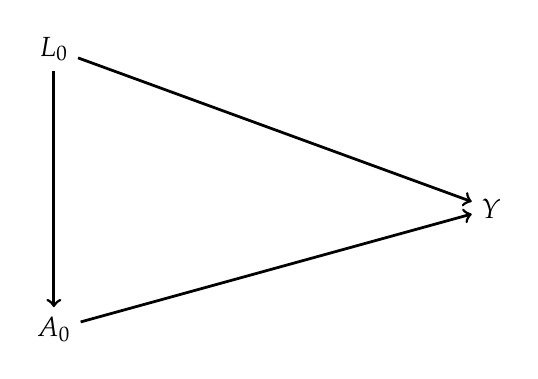
\begin{tikzpicture}

% nodes %
\node[text centered] (l0) {$L_0$};
\node[below = 3 of l0, text centered] (a0) {$A_0$};
\node[below right = 1.5 and 5 of l0, text centered] (y) {$Y$};

% edges %
\draw[->, line width= 1] (a0) --  (y);
\draw[->, line width= 1] (l0) --  (a0);
\draw[->, line width= 1] (l0) --  (y);

\end{tikzpicture}
\caption{Causal graph}
\end{figure}

    \subsection{Time dependent
confounding}\label{time-dependent-confounding}

So far we have considered the time fixed context in which treatment and
confounders take on a single value. It was sufficient to block the "back
door" path between the treatment and outcome by conditioning on the
confounding variable(s). In the headache example, the causal effect of
ibuprofen on headache alleviation was confounded by sex. For most
people, sex is a time-fixed covariate because it does not change value
over time. To broaden the setting to a time dependent context, we adopt
the canonical example of the causal effect of Zidovudine (AZT) on
mortality amongst human immunodeficiency virus (HIV)-infected subjects
\citet{Hernan2000}. In this example, subjects are measured at baseline
\(t = 0\) and at subsequent visits. In each visit the patient's CD4
lymphocyte count is measured and a treatment decision made. Survival at
the end of follow-up is a binary outcome equal to 1 if the patient has
died and 0 otherwise. \linebreak

The time-fixed notation can be extended to include subject histories for
time varying variables. Treatment and covariate histories up to visit
\(k\) are can be represented by an overhead bar. For example,
\(\bar X_{k} = \{X_{0}, \hdots, X_{k}\}\) represented the vector of
treatment decisions while \(\bar Z_{k} = \{Z_{0}, \hdots, Z_{k}\}\)
represents the vector of measurements on the time dependent-confounder
\(Z\). Time-fixed covariates like sex, or covariates which change
linearly over time like age are tyically recorded at baseline
(\(t = 0\)) and we denote the collection of baseline covariates as
\(V_{0}\). The outcome of interest at the end of follow-up is mortality
\(Y\) which is a binary variable taking the value \(1\) if the patient
is dead and \(0\) otherwise. \linebreak 

Just as in the time-fixed case, time-dependent confounders lead to
spurious associations between \(X\) and \(Y\) through a "back door" path
between \(X\) and \(Y\) through \(L\). To estimate a causal effect it is
necessary to block or screen off this path by conditioning or
stratifying on the confounding variables. Figure ? gives an example of
this in the time dependent case for two periods (\(t = 0, 1\)). In the
first period a treatment decision is made based on the measured
confounder \(Z_0\). In the second period (\(t = 1\)) a new treatment
decision is made based on both \(Z_0\) and \(Z_1\). Conditioning on
\(\bar Z\) under this DAG leads to a consistent estimate of the causal
effect because doing so blocks all paths between \(X_0\) and \(X_1\) and
\(Y\) except the causal path of interest. \linebreak

However, the time-dependent context also admits structures like the
middle pane of figure ? with the addition of a causal relationship
between \(X_0\) and \(Z_1\). It is now possible for current treatments
to be a determinant of future confounders which are in turn determinants
of future treatment \citet{Robins2000a}. As a result the effect of
\(A_0\) on \(Y\) is mediated through \(L_1\) in the path
\(A_0 \rightarrow L_1 \rightarrow Y\). Blocking this path by
conditioning on \(Z\) also blocks some portion of the effect of \(A_0\)
on \(Y\) and will lead to a biased estimate. \linebreak

A second danger in the time-dependent context arises when \(Z\) is a
common effect of treatment and an unmeasured variable \(U\) which also
influences the outcome \(Y\). There is no direct association Figure ?
shows the same two structures with the addition of a an unmeasured
variable \(U\) which influences \(Z\) and \(Y\). Conditioning on \(Z\).
Selection bias precludes unbiased estimation \citet{Hernan2004}. There
is a mediating relationship between \(A\) and \(Z\) in which case there
is a spurious relationship between \(A\) and \(Y\) again? This is less
inuitive and so examples are best according to \citet{Cole2010}. We can
say that Z is a common effect of A and U, once we condition on Z we
create a dependence of A on U. U is a cause of Y and hence there is an
association between A and Y. This association is present even when there
is no direct causal path between A and Y. \linebreak

Conclusion, 1) clearly a different technique is required for analysis 2)
the nature of time dependent case needs to be described fully enough to
explain why we choose the simulation algorithm that we choose and any
holes in it. In subsequent sections our choice of simulation algorithm
will be motivated by the structure of time dependent confounding as well
as the viability of introducing positivity violations which are
propogated through the time dependent structure. Explain meaning of a
collider and that a collider that is conditioned on will not block
confounding. Essentially with this kind of data we cannot use
confoudning or stratification methods.

\begin{itemize}
\tightlist
\item
  introduce survival analysis?
\item
  Intuition from Pearl 2009 book pp. 17 on sprinklers.
\item
  Simpson's paradox linked to making comparisons within strata
\item
  explain that we are often interested in parsimnonious models so cannot
  have all covariates \(U\) that will create associations between \(X\)
  and \(Y\)
\item
  explain why we do not need to worry about the path between A\_0 and
  A\_1
\item
  explain why mediation is likely to occur in example.
\item
  explain why saturated models cannot be used because they will have
\item
  inituitive examples of selection bias.
\item
  Saturated models are not an option because they would be
  computationally intensive and so we use parametric models which also
  links to positivity because we smooth over zeroes in certain strata.
\end{itemize}

    \begin{figure}

\begin{minipage}{.2\textwidth}

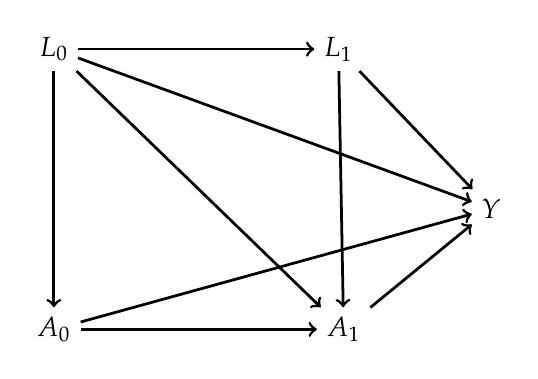
\begin{tikzpicture}

% nodes %
\node[text centered] (l0) {$L_0$};
\node[below = 3 of l0, text centered] (a0) {$A_0$};
\node[right = 3 of l0, text centered] (l1) {$L_1$};
\node[right = 3 of a0, text centered] (a1) {$A_1$};
\node[below right = 1.5 and 5 of l0, text centered] (y) {$Y$};

% edges %

%L0%
\draw[->, line width= 1] (l0) --  (l1);
\draw[->, line width= 1] (l0) --  (a0);
\draw[->, line width= 1] (l0) --  (a1);
\draw[->, line width= 1] (l0) --  (y);

%A0%
\draw[->, line width= 1] (a0) --  (a1);
\draw[->, line width= 1] (a0) --  (y);

%L1%
\draw[->, line width= 1] (l1) --  (a1);
\draw[->, line width= 1] (l1) --  (y);

%A1%
\draw[->, line width= 1] (a1) --  (y);

\end{tikzpicture}

\end{minipage}
\hspace{5cm}% NO SPACE BETWEEN \end \hspace and \begin!
\begin{minipage}{.2\textwidth}

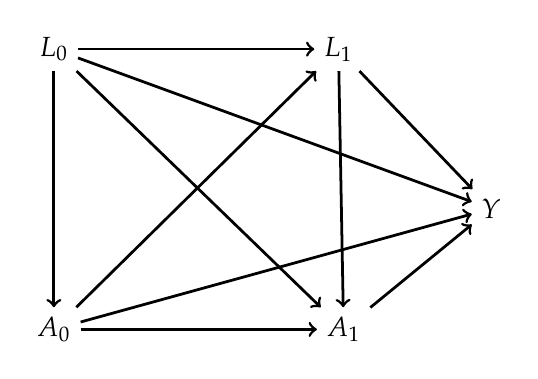
\begin{tikzpicture}

% nodes %
\node[text centered] (l0) {$L_0$};
\node[below = 3 of l0, text centered] (a0) {$A_0$};
\node[right = 3 of l0, text centered] (l1) {$L_1$};
\node[right = 3 of a0, text centered] (a1) {$A_1$};
\node[below right = 1.5 and 5 of l0, text centered] (y) {$Y$};

% edges %

%L0%
\draw[->, line width= 1] (l0) --  (l1);
\draw[->, line width= 1] (l0) --  (a0);
\draw[->, line width= 1] (l0) --  (a1);
\draw[->, line width= 1] (l0) --  (y);

%A0%
\draw[->, line width=1] (a0) --  (a1);
\draw[->, line width=1] (a0) --  (l1);
\draw[->, line width=1] (a0) --  (y);

%L1%
\draw[->, line width= 1] (l1) --  (a1);
\draw[->, line width= 1] (l1) --  (y);

%A1%
\draw[->, line width= 1] (a1) --  (y);

\end{tikzpicture}

\end{minipage}
\caption{Figure 1 DAG} \label{fig:fig2}
\end{figure}

    \begin{figure}

\begin{minipage}{.2\textwidth}

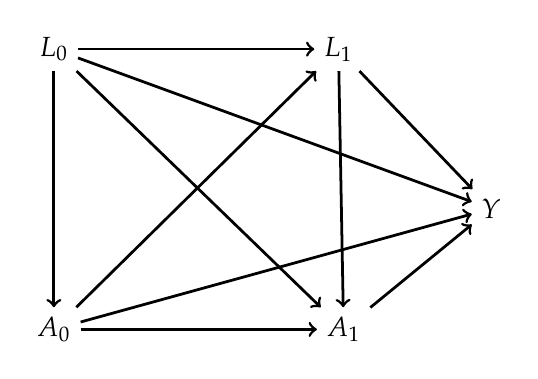
\begin{tikzpicture}

% nodes %
\node[text centered] (l0) {$L_0$};
\node[below = 3 of l0, text centered] (a0) {$A_0$};
\node[right = 3 of l0, text centered] (l1) {$L_1$};
\node[right = 3 of a0, text centered] (a1) {$A_1$};
\node[below right = 1.5 and 5 of l0, text centered] (y) {$Y$};

% edges %

%L0%
\draw[->, line width= 1] (l0) --  (l1);
\draw[->, line width= 1] (l0) --  (a0);
\draw[->, line width= 1] (l0) --  (a1);
\draw[->, line width= 1] (l0) --  (y);

%A0%
\draw[->, line width=1] (a0) --  (a1);
\draw[->, line width=1] (a0) --  (l1);
\draw[->, line width=1] (a0) --  (y);

%L1%
\draw[->, line width= 1] (l1) --  (a1);
\draw[->, line width= 1] (l1) --  (y);

%A1%
\draw[->, line width= 1] (a1) --  (y);

\end{tikzpicture}

\end{minipage}
\hspace{5cm}% NO SPACE BETWEEN \end \hspace and \begin!
\begin{minipage}{.2\textwidth}

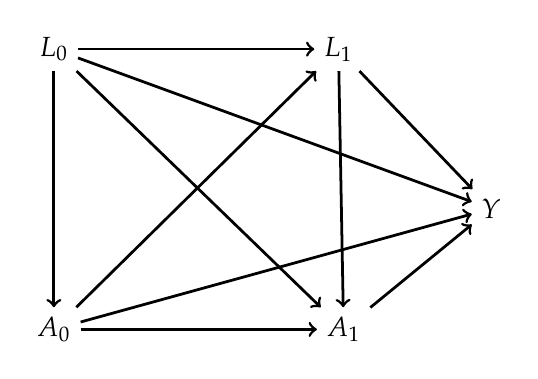
\begin{tikzpicture}

% nodes %
\node[text centered] (l0) {$L_0$};
\node[below = 3 of l0, text centered] (a0) {$A_0$};
\node[right = 3 of l0, text centered] (l1) {$L_1$};
\node[right = 3 of a0, text centered] (a1) {$A_1$};
\node[below right = 1.5 and 5 of l0, text centered] (y) {$Y$};

% edges %

%L0%
\draw[->, line width= 1] (l0) --  (l1);
\draw[->, line width= 1] (l0) --  (a0);
\draw[->, line width= 1] (l0) --  (a1);
\draw[->, line width= 1] (l0) --  (y);

%A0%
\draw[->, line width=1] (a0) --  (a1);
\draw[->, line width=1] (a0) --  (l1);
\draw[->, line width=1] (a0) --  (y);

%L1%
\draw[->, line width= 1] (l1) --  (a1);
\draw[->, line width= 1] (l1) --  (y);

%A1%
\draw[->, line width= 1] (a1) --  (y);

\end{tikzpicture}

\end{minipage}
\caption{Figure 1 DAG} \label{fig:fig2}
\end{figure}

    \subsection{Inverse Probability of Treatment
Weighting}\label{inverse-probability-of-treatment-weighting}

\begin{itemize}
\tightlist
\item
  Dangers associated with startification and controlling for methods
  highlighted already explain why we need other methods - explain a few
  of these like G-estimation, SNTM etc.
\item
  creates a pseudo-population in which we have something similar to an
  experimental setting
\item
  Because we need weights this means we need a model for the weights -
  model can be non parametric or parametric depending on data used.
\item
  Contrast IPTW methods with stratification methods.
\end{itemize}

\citet{Horvitz1952}

Recap of issues with time dependent confounding. Introduce IPTW as a
means of dealing with these issues. Areas where IPTW has been used (time
dependent confounding, comparing dynamic regimes, missing data)

Inverse probability of treatment weighting is a technique that
re-weights subject observations to a population where assignment of
treatment is at random. An early example of this technique is the
\citet{Horovitz1952} weighted estimator of the mean. In the context of
marginal structural models, a weight is calculated for each subject
which can be thought of informally as the inverse of the probability
that a subject receives their own treatment \citet{Robins2000}. The
result of applying these weights is to re-weight the data to create a
pseudo-population in which treatment is independent of measured
confounders \citet{Cole2008}. The resulting pseudo population no longer
has a time dependent confounding problem and the causal relationship
between A and Y can be estimated using naive methods like regression
without adjusting for confounding because it is no longer present.
Crucially, in the pseudo population the counterfactual probabilities are
the same as in the true study population so that the causal RD, RR or OR
are the same in both populations \citet{Robins2000}.

\[w_{t,i} = \frac{1}{\prod_{\tau=0} ^ t p_{\tau} (A_{\tau, i}\ |\ \bar A_{\tau-1, i}, \bar L_{\tau, i})}\]

stabilized weights
\[sw_{it} = \frac{\prod_{\tau=0} ^ t p_{\tau} (A_{\tau, i}\ |\ \bar A_{\tau-1, i})} {\prod_{\tau=0} ^ t p_{\tau} (A_{\tau, i}\ |\ \bar A_{\tau-1, i}, \bar L_{\tau, i})}\]

The use of IPTW is valid under the four assumptions of consistency,
exchangeability, positivity and no misspecification of the model
\citet{Cole2008}.

Informally a patients weight through visit k is proportional to the
inverse of the probability of having her own exposure history through
visit k (Cole and Hernan 2008)

Explain why this method does appropriately adjust for \textbf{measured
time varying} confounders affected by prioir exposure.

The weight is informally proportional to the participants probability of
receiving her own exposure history

As these weights have high instability we need to stabilize them. The
unstabilized weights can be driven by only a small number of
observations. Under time dependent confounding it may still be possible
to recover the causal effect of \(A\) on \(Y\) by the method of Inverse
Probability of Treatment (IPT) weihting. How does this work?

\begin{itemize}
\tightlist
\item
  true weights are unknown but can be estimated from the data.
\item
  \(A_t\) is no longer affected by \(L_t\), and crucially the causal
  effect of \(\bar A\) on \(Y\) remains unchanged
\end{itemize}

Be more specific about what is contained in the weights. The denominator
depends on the measured confounders \(L\) the numerator does not.

\begin{itemize}
\tightlist
\item
  weighted regression and MSM are equivalent.
\end{itemize}

Point out that we need baseline variables in the conditional statments
in the num and denom of the weights otherwise we break the relationship
between outcome and baselines in the new pseudo-population. If the
baseline variables are not confounders, then we do not want to break
this relationship. Baseline covariates also help to stabalize the
weights (how?)

importantly, changing the relationship between L and A, won;t change the
relationship between L and Y. This means that an intervention in \(A\)
does not affect the relationship between \(L\) and \(Y\). So we remove
the link between \(L\) and \(A\) and assign to \(A\) the value of
treatment on or off. Once we place the patient on treatment, regardless
of the relationship which had existed before hand between the covariate
and treatment, a new relationship between \(A\) and \(Y\) exists in
which the covariate has no say.

\subsubsection{Applications of IPTW}\label{applications-of-iptw}

Different from application of MSMs - IPW is a technique which has been
applied to MSMs - i.e. MSMs are on example of how IPTW can be used.

    \subsection{Assumptions}\label{assumptions}

This section presents a more formal discussion of the key assumptions
underlying MSMs. Most attention will be given to positivity. Conditions
under which IPTW work are largely untestable (westreich 2012)

\subsubsection{Exchangeability}\label{exchangeability}

\[Y_{x} \perp\!\!\!\perp X\]

\subsubsection{Consistency}\label{consistency}

\citet{Cole2009} \citet{Pearl2010}

\subsubsection{No model mispecification}\label{no-model-mispecification}

\subsubsection{No measurement error}\label{no-measurement-error}

\subsubsection{Positivity.}\label{positivity.}

The final assumption underlying MSMs, and the central topic of this
thesis, is the positivity assumption. MSMs are used to estimate average
causal effects in the study population, and one must therefore be able
to estimate the average causal effect in every subset of the population
defined by the confounders \citet{Cole2008}. The positivity assumption
requires that there be exposed and unexposed individuals in every strata
of the confounding covariates. For example, when treatment is Zidovudine
and CD4 count is the confounder, there must be a positive probability of
some patients being exposed and unexposed at every level of CD4 count.
Positivity can be expressed formally as \(Pr(A=a\ |\ L) > 0\) for all
\(a \in A\), which extends straightforwardly to the time dependent case
where the positivity assumption must hold at every time step conditonal
on previous treatment, time dependent confounders and any baseline
covaraiates:

\[Pr(A_{it}=a_{it}\ |\ L_{it}, A_{i, t-1}, V_{i0}) > 0\]

Models for the risk \(P(Y=1\ |\ A=a, L=l)\) are commonly studied in
epidemiological applications. Applying basic probability rules reveals
that the risk can be re-written with the term \(Pr(A=a\ |\ L=l)\) in the
denominator:

\[P(Y=1\ |\ A=a, L=l) = \frac{P(Y=1, A=a, L=l)}{Pr(A=a, L=l)} = \frac{P(Y=1, A=a, L=l)}{Pr(A=a\ |\ L=l)Pr(L=l)}\]

This model is only estimable when \(Pr(A=a\ |\ L=l) \neq 0\). Therefore,
when positivity does not hold it is not possible to estimate the model.
In the context of MSMs a similar problem emerges. Although weighting via
IPTW allows naive estimation of (?) without including the confounders,
the weights in (?) involved the term \(Pr(A=a\ |\ L=l)\) in the
denominator. This means that the weights are inestimable whenever
positivity is violated. In order to estimate the causal effect of \(A\)
on \(Y\), weights must be estimable in every subset of the population
otherwise the average causal effect in the study population cannot be
estimated. \linebreak

In practice, positivity can arise when random zeroes or structural
zeroes are present in some levels of the confounding covariates. Random
zeroes arise when, by chance, no individuals or all individuals, receive
treatment within a certain strata as defined by the covariates. For
example, \citet{Cole2008} studies positivity violations in individuals
in strata defined by CD4 count and viral load. By increasing the levels
of CD4 count the chances of random zeroes also increases and
\citet{Cole2008} show that the IPT weights rapidly lose their stability
with the consequence that causal effects are no longer estimable.
Researchers applying IPTW methods must actively check that there are
both treated and untreated individuals at every level of their
covariates within cells defined by their covariates because parametric
methods will smooth over positivity violations and not provide any
indication of nonpositivity. Increasingly refined covariates are
attractive because they provide better control of confounding, but the
point that \citet{Cole2008} make is that this control needs to be traded
off against increased occurence of random zeroes and subsequent
instability of IPT weights. \linebreak

More relevant to this thesis are violations of the positivity assumption
due to structural zeroes. These occur when an individual cannot possibly
be treated or if an individual is always treated within some levels of
the confounding covariate, as is the case in the clinical protocol
example motivating this thesis. Several studies give examples of
structural violations of the positivity assumption in epidemiological
contexts. In \citet{Cole2008} structural zeroes arise when the health
effects due to exposure to a chemical are confounded by health status
proxied by being at work. If individuals can only be exposed to the
chemical at work then all individuals not at work will be unexposed. A
second example is liver disease as a contraindication of treatment. If
individuals with liver disease cannot be treated then all individuals in
the "liver disease = 1" strata will be untreated. In \citet{Messer2010}
structural zeroes arise in the context of rates of preterm birth and
racial segregation, whereas \citet{Cheng2010} find structural zeroes in
the context of fetal position and perinatal outcomes. Our motivating
example is most closely related to liver disease as a contraindication,
except that the clinical protocols require that patients with low CD4
count always be treated instead of never being treated, as in the case
in the liver disease example. \linebreak

Although in many epidemiological settings the positivity assumption is
guaranteed by experimental design, studying positivity violations is
relevant because, as our own motivating example and the examples above
suggest, structural violations do occur, and random zeroes are always
possible especially at finer levels of confounding covariates. Studying
the finite sample propoerties of MSMs under violations to positivity is
therefore an important issue which is yet to be dealt with
systematically in the literature. As \citet{Westreich2010} points out,
positivity violations, positivity violations by a time varying
confounder pose an analytic challenge and they suggest g-estimation or
g-computation may be a way forward. A good start to dealing with the
time varying confounder case is to see how well MSMs work when
positivity is violated. This is also a novelty of this thesis.

\begin{enumerate}
\def\labelenumi{\arabic{enumi}.}
\setcounter{enumi}{5}
\tightlist
\item
  estimated weights with a mean far from one, or very extreme values
  indicate either non-positivity or model mispecification of the weight
  model.
\item
  It is not always true that we want more finely tuned covariates for
  confounder control because the bias and variance of the effect
  estimate may increase with the number of categories. This is similar
  to the positivity masking example.
\item
  Our results are equally valid for other circumstances in which
  positivity may arise.
\item
  Also think about how the number of categories of exposure increases
  the chance that one level of exposure will have a positivity.
\item
  Westreich and Cole 2010 have suggested that methodological approaches
  are needed to weigh the resultant biases incurred when trading of
  confounding and positivity. The framework we use is flexible enough to
  allow this in a simulation setting.
\end{enumerate}

If the structural bias occurs within levels of a time-dependent
confounder then restriction or censoring may lead to bias whether one
uses weighting or other methods (Cole and Hernan 2008). In fact,
weighted estimates are more sensitive to random zeroes (Cole, Hernan,
2008) Introducing violations of positivity can be achieved by censoring
observations.

But to give an intuitive example, think about how it links back to a
situation where sicker patients receive treatment compared to others. So
in the "sick" strata of the CD4 count \textbf{ALL} patients receive
treatment which inflates the IPTW. This also affects how we think about
the associational versus causal models. The causal effect might be 50/50
but because sicker patients get treatment the mortality ratio in the
treated group is likely to be higher.

The trade-off between positivity and confounding bias is emphasized in
Cole2008

Why is practicality important? Cole paper highlights practical advice to
practictioners. positivity can be violated in a practical setting
because of two few strata, it can be the result of protocols in a
clinical setting and it can be seen as a trade-off between
exchangeability (and we need more measured predictors to maintain
exchangeability) and positivity where more predictors leads to more
likely a zero problem.

\begin{itemize}
\tightlist
\item
  Dynamic stratgies evaluated using MSMs will have rules like, start
  treatment if CD4 falls below a certain threshold. See Didelez
  presentation on this
\item
  Explain that there is positivity in estimation of the structural model
  and also in the weight model. The reason why positivity is more
  important in the weight model is because when the weights are unstable
  the estimates can be very wrong as a result.
\end{itemize}

    Have been used for missing data problems. see pp.442 of Hernan,
Brumback, Robins 2001 for a list of papers linked to this

A model that parameterises \(P(Y\ |\ do(A=a))\) is called a marginal
structural model (MSM) as it is marginal over any covariates and
structural in the sense that it represents an interventional rather than
observational model.

    \newpage

    \section{Simulating from marginal structural
models}\label{simulating-from-marginal-structural-models}

In order to assess the effect of violations of the positivity
assumption, we adopt the algorithm of \citet{Havercroft2012} for
generating longitudinal data. This algorithm is suitable for several
reasons. Firstly, it allows us to simulate observational data from a
known MSM so that when positivity violations are introduced we can
compare estimates under positivity violations with those from the known
MSM. Secondly, we can simulate data with observational structure
including selection bias which is particulalry important for survival
models. Thirdly, this algorithm is suitable for noncollapsible models
including survival models. And finally the algorithm needs to be
flexible enough to allow us to introduce positivity violations. In this
section we describe this algorithm and the properties that make it
suitable for analysing the effect of positivity violations on MSMs.

From the point of view of simulating from a marginal structural model,
In a nutshell, we need a simulation algorithm that allows us to simulate
discrete time longitudinal data in which A affects Y, and so does L and
L affects A. The most direct way of doing this would be the red line in
the DAG. But this won't do in our case. The Havercroft and Didelez
algorithm is useful because it allows us to break the relationship
between L and A. We need to do this in such a way that we do not change
the relationship between Y and L, although we are not so interested in
this relationship because it is the least interesting of the
relationships in the diagram.

\subsection{Specific MSM}\label{specific-msm}

Testing positivity violations requires generating data from a known MSM.
For example, suppose that the chosen MSM was
\(P(Y\ |\ do(a)) = \alpha + \beta a\), then the observational data from
which this is derived would be \(Y\), \(A\) and \(L\). The simulation
needs to allow \(\beta\) to be estimated from only that observational
data. In order to simulating from a specific MSM we need to generate
observational data in such a way that it conforms to a specific MSM. For
instance, one specific MSM could be written as
\(P(Y\ |\ do(a)) = \alpha + \beta a\). However, we never see this so we
need to generate data in such a way that we get this model from
observational data and that we can then return to it.

\subsection{observational structure}\label{observational-structure}

The observational structure needs to include the central parts of time
dependent confounding - in particular Y and A are common effects of U
which creates a confounding relationship. We also need selection bias,
some models like hazard ratios have a built in selection bias so this is
particularly important.

\subsection{noncollapsibility}\label{noncollapsibility}

Collapsibility means there is no incompatibility between the marginal
model and the conditional distributions used to simulate the data.
Provide example of this. Explain how this affects the simulation
algorithm. Especially hazard ratios which are non-collapsible.

\subsection{simulation models}\label{simulation-models}

\begin{itemize}
\item
  Bryan 2004: fixes the vector L at the beginning which means A never
  affects L which don't make no sense.
\item
  Westreich 2 papers
\item
  others.
\item
  why we choose the havercroft one
\item
  What is the advantage of havercroft over Bryan.
\end{itemize}

Models are noncollapsible when conditioning on a covariate
\textbf{related to the outcome} changes the size of the estimate even
when the covariate is unrelated to the exposure. Illustrate why this
happens with survival models.

Exlain why survival models are noncollapsible and why the CDF method
based on U is how we overcome this. Survival models are non-collapsible
because

Hazard rations

Hazard rations have built in selection bias when we consider period
specific hazard ratios. This is because it is selective on patients
reaching the time period in question.

The parameter of interest could be expected survival or the five year
survival probability

This is particularly important because collapsibility and confounding
are often treated as identical concepts when in fact they are not.
\citet{Greenland1999}

generate L and A based on U. Transform U to obtain Y. Trick is to get to
Y and this comes through properties of the CDF.

The confounding structure occurs because there is a relationship between
A and Y confounded through L through U? Y and A are common effects of U
which creates an association between A and Y other than the causal
association we want to study in the MSM - refer to structural bias
paper.

The true MSM that we want to resolve using IPTW needs to take a known
form. This is the hazard function - which is of a form that we choose in
advance. Survival models are non-collapsible. Hence we cannot eaily
simulate from them - so why are we able to do it in this case?

Need to specify what the MSM is, give an example of it as a hazard
function. Survival is completeley determined by the hazard function.

We could adjust for confounding y blocking all back door paths. SO need
to explain what the back dorr path is. Need to explain intuitevely why
it is there.

U allows us to get any distribution we like for Y marginal over
covariates, WOuld L itself allows this? probably not. We can somehow get
from this the subjects counterfactual survival time.

\subsection{role of u - what problem does u
solve.}\label{role-of-u---what-problem-does-u-solve.}

As they point out, it is not always obvious how to simulate data from a
given MSM because of noncolapsibility. The DAG in figure 1 represents
the causal system in question.

Ultimately we need an algorithm which exhibits the observational
qualities we want and, at the same time, comes from a given MSM.. We
need an algorithm which exhibits time dependent confounding. We need the
model to take a known form so we specify in advance what the parameters
should be.

Importantly, this expression on the left hand side has unobserved
counterfactuals, but the right hand side has only observed quantities
which would be observed in an actual observational study.

non-collapsibility is an unresolved issue here. So even if we
investigate positivity we can still only do so for collapsible models?

Equivalent way of motivating dividing the joint distribution by
Pr(A\textbar{}L) is through IPTW.

Collapsability comes in because we cannot collapse a model conditional
on L into one conditional on only A. Why do we need to get rid of L to
get the correct MSM?

Problem is that conditional distributions one might use to draw the
simulated data are not compatible with the desired properties of the
marginal model. Is this collapsibility?

Following the math through, we want to end up with the correct
coefficient, having L in there does not matter really. The important
point is to resolve the correct, causal parameter on a

How does selection bias relate to \(U\)?

Explain why the algoritm allows positivity to be propagated throught the
patients history. Always linking back to positivity

The simulating procedure needs to allow us to specifiy a particular MSM,
while at the same time capturing the characteristics of observational
data.

\begin{enumerate}
\def\labelenumi{\arabic{enumi}.}
\item
  derive relationship between MSM and DAG and the correct conditional
  distributions. Follows from truncated factorisation why we can et
  P(Y\textbar{}do(a))
\item
  simulating from a chosen MSM
\item
  creating a confounding relationship
\item
  only have the data and observed outcomes, not the counterfactuals.
\item
  Fixing relationships.
\item
  think of this process as if we had fixed a treatment vector in
  advance. consistency assumption.
\item
  Relationship between A and L should be observational and a confounding
  relationship
\item
  U is breaking the relationship between L and Y, important for
  positvity.
\item
  Don't care about the relationship between L and Y
\item
  HD 2012, with Pearl and truncated factorization formula, show that it
  is possible to link the counterfactual represented by
  \(P(Y\ |\ do(a))\) to observattional data generated in an
  observational way. But the problem arises when the model is
  non-collapsible or non-linear.
\end{enumerate}

In the one shot case we set A = 1/0 because we are interested in the
outcome under either of these treatment scenarios. In the time dependent
case, A is a vector of 0s and 1s and we want to pretend that we decide
in advance that the whole vector A is specified. But A and L have a
complex interplay in an observational setting. So we want to pretend
that A (a vector of 1s and 0s) is set in advance but at the same time
have the observational structure for A and L.

The relationship between Y and L is then dependent on A. There is no
relationship between A and U because of the set-up in the DAG. The
variable L blocks this relationship.

In their paper \citet{Havercroft2012} develop an algorithm that allows
simulating data that corresponds to a particular parameterisation of an
MSM. This algorithm provides the bedrock of the simulation structure
considered in this thesis. Figure 1 represents the system under
consideration. The DAG in figure 1 represents the one-shot
non-longitudinal case. Factorising the joint distributions of the
variables in figure 1 yields

\[P(U,\ L,\ W,\ A,\ Y) = P(W)P(U)P(W)P(L\ |\ U)P(A\ |\ L,W)P(Y\ |\ U,A)\]

Where, following definition 1.1 we delete \(P(A\ |\ L,W)\), a
probability function corresponding to \(A\), and replace \(A=a\) in all
remaining functions

\[ P(U, L, W, Y\ |\ do(A=a)) =
  \begin{cases}
    P(U)P(L\ |\ U)P(Y\ |\ U,A = a) & \quad \text{if } A = a\\
    0  & \quad \text{if } A \neq a\\
  \end{cases}
\]

The goal is to simulate from a particular MSM. This means parameterising
\(P(Y\ |\ do(A=a))\). Applying the law of total probability over \(W\),
\(U\) and \(L\) yields

\[P(Y\ |\ do(A=a) = \sum_{w, u, l} P(W)P(U)P(L\ |\ U)P(Y\ |\ U, L, A=a) = \sum_{u, l} P(U)P(L\ |\ U)P(Y\ |\ U, L, A=a)\]

Making use of the fact that
\(P(L, U) = P(L\ |\  U)P(U) = P(U\ |\ L)P(L)\) and summing over either W
and U or W and L yields

\[P(Y\ |\ do(A=a) = \sum_{l}P(Y\ |\ L, A=a)P(L) = \sum_{u} P(Y\ |\ U, A=a)P(U))\]

If we can find suitable forms for either \(P(Y\ |\ L, A=a)\) and
\(P(L)\) or \(P(Y\ |\ U, A=a)\) and \(P(U)\) that correspond to the MSM
\(P(Y\ |\ do(A=a)\), then, given suitable values for \(A, L, U\) it will
be possible to simulate from the chosen MSM.

use the phrase, "in words ...." to make something more understandable.

Choosing a functional form for \[P(Y\ |\ do(A=a)\] depends on
convenience. We need a functional form that can be easily represented by
\(P(Y\ |\ L, A=a)P(L)\). non-linear functions will be hard to work into
the analysis.

U \textasciitilde{} U{[}0, 1{]} is a good choice because we can usethe
CDF of Y because U{[}0, 1{]} is always between 0 and 1

General health is patient specific but comes from a clear distribution
and has a nice medical interpretation. In contrast L would be more
difficult to include. It is better as a function of U than a value in of
itself.

Don't forget basics like knowing what the true model is and therefore
being able to compare the true model with the results. Explain why
simulations work in a general sense don't take it for granted.

    The aim is to be able to simulate the survival function of a desired MSM
under the intervention \(do(\bar a)\)

Several studies have developed algorithms for simulating data from
marginal structural models in the presence of time dependent
confounding. An early example is \citet{bryan2004} who study estimators
of the causal effec of a time dependent treatment on survival outcomes.
They compare naive estimators with IPTW and a treatment orthogonalized
estimator which is also developed in the paper. This study shares
similarities with \citet{Havercroft2012}

\begin{itemize}
\item
  stay on treatment after treatment starts
\item
  treatment regime is determined by t* (starting point of treatment
  because it is a vector of \{0, 0, 0, 1, 1, 1\}
\item
  they motivate a logistic model for the haxard function, they use a
  discrete equivalent to the hazrd function (link to citation about
  farington study.)
\item
  the survival time U is directly linked to the survival outcome
  -\textgreater{} here it is good to provide more inuition.
\item
  need to understand why it is linked.

  Work that proposes a different method to solve the same problem. Work
  that uses the same proposed method to solve a different problem. A
  method that is similar to your method that solves a relatively similar
  problem. A discussion of a set of related problems that covers your
  problem domain.
\end{itemize}

These previous studies have lacked a systematic investigation of
positivity violations in a simulation setting. It is unknown, for
example, how large an effect a violation of positivity has and how it is
affected by the sample size, threshold etc etc.

\begin{enumerate}
\def\labelenumi{\arabic{enumi}.}
\item
  marginal structural models literature
\item
  Simulating from marginal structural models
\item
  positivity
\item
  connect limited work on simulating from models to positivity
\item
  Explain why we choose the Havercroft simulation of the others,
  specifically why it helps us to incorporate violations of positivity
  in our analysis.
\end{enumerate}

Several studies have considered simulation from margial structural
models. The finite-sample properties of marginal structural proportional
hazards models has been considered by \citet{Westreich2009}.

\begin{itemize}
\tightlist
\item
  What is their focus?
\item
  how do they simulate
\item
  what do they find (in terms of MSE, SE, etc.
\item
  how does it differ from HD (2012)
\end{itemize}

Young etal (2014) also provide a simulation algorithm for simulating
longitudinal data from a known Cox MSM.

Comparing IPW and standard regression based estimates in the absence of
model misspecification. This allows for complete isolation of any type
of bias. This approach involves simulating data from a standard
parametrization of the likelihood and solving for the underlying Cox MSM

we describe an approach to Cox MSM data generation that allows for a
comparison of the bias of IPW estimates versus that of standard
regression-based estimates in the complete absence of model
misspecification

Cole (2008) for more of a discussion about positivity, with an actual
observed data example. While Cole (2008) have looked at positivity in an
observational setting, to our knowledge no study has looked at
positivity violations within a simulation setting.

Cole and Hernan 2008 have examined the four assumptions underlying IPW
using a study on real data from the HAART SWISS study.

\begin{enumerate}
\def\labelenumi{\arabic{enumi}.}
\tightlist
\item
  2 paper on simulation + Bryan paper - why this simulation method is
  different from other sim papers
\item
  related work - Judea pearl, Robins, econometrics, related and broader
  literature on MSM
\item
  positivity long discussion in Hernan and cole and the warnings but no
  simulation study in that paper. They study the positivity but not the
  effect and there is nothing in the havercroft paper on this either.
\end{enumerate}

\begin{itemize}
\item
\item
  Major point is that there are a number of ways of simulating from
  marginal structural models. But, we need one where we can mess with
  the positivity. Other methods are not suitable for this.
\item
  G formula simulation
\item
  exposure, confounder feedback loop
\item
  treatment
\item
  outcome variable
\item
  causal effect of the treatment variable on the outcome.
\item
  external intervention
\item
  Explain the do notation, and what presicely is meant in the case\\
\item
  used to estimate the joint effect of time dependent treatments on
  survival
\item
  Need to stronly link the time dependent confounding to the MSM, do we
  choose this class of models because of their relationship with time
  dep confounding? Yes, marginal strictural models are used with TDC
\item
  The causal graph helps (according to Pearl pp. 40) to bridge
  statistics into causality
\item
  There is a key part to this, which is that we do not observe
  confounding, this seems to be what motivates the use of the MSM class
  of models.
\item
  Counterfactuals need to be addressed here to make it clear this is not
  the purpose of the thesis.
\item
  Robins (2000) have demonstrated that in the presense of time dependent
  confounders, standard approaches for asjusting for confounding are
  biased.
\item
  A covariate that is a risk factor for, or predictor of the event of
  interest (Y) (from Robins 2000). This defines a time dependent
  covariate
\item
  And also past exposure determines the level of the covariate.
\item
  Works under a set of assumptions (consistency, exchanchability,
  positivity and no mispecification of the model used to estimate the
  weights
\item
\end{itemize}

    \section{Violations of Positivity}\label{violations-of-positivity}

The motivation for using the algorith of \citet{Havercroft2012} is that
we have control over how \(L\) affects \(Y\), so we can itroduce
positivity using a threshold. In other algorithms there would be a
direct link between \(L\) and \(Y\), this would be a problem because
altering treatment decisions based on \(L\) would affect \(Y\)
directly.\\
- creating an artificial population in which positivity is violated in
specific ways.

\subsection{Extended discussion of algorithm linking to
positivity}\label{extended-discussion-of-algorithm-linking-to-positivity}

As described in the introduction, one assumption of the model is that
there is a non-zero probability of the event occuring at every startum
of the covariate.

\begin{itemize}
\tightlist
\item
  When previous covariates like CD4 count are strongly associated with
  treatment the probabilities in the denominator of the ustabilized
  weights may vary greatly. Because we are foricing positivity by using
  a treatment rule when L falls below a threshold and A is then eaual to
  one, we create a strong association between A and L -\textgreater{}
  hence the unstabilized weights would vary. (Robins et al 2000 pp. 553)
\item
  present the algorithm again with positivity violations.
\end{itemize}

    \section{Application}\label{application}

\subsection{Data Structure}\label{data-structure}

We wish to simulate survival data in discrete time \(t = 0, \dots, T\)
for \(n\) subjects. At baseline \(t=0\) all subjects are assumed to be
at risk of failure so that \(Y_0 = 0\). For each time period
\(t = 0, \dots, T\) a subject may either be on treatment, \(A_t = 1\),
or not on treatment, \(A_t = 0\). All patients are assumed to be not on
treatment before the study begins. Once a patient commences treatment,
they remain on treatment in all subsequent periods until failure or the
end of follow-up. In each time period \(L_t\) is the value of a
covariate measured at time \(t\). In the simulated data, \(L_t\) behaves
in a similar manner to CD4 counts such that a low value of \(L_t\)
represents a more severe illness and hence a higher probability of both
tratemnt and failure in the following period. In addition to \(L_t\),
the variable \(U_t\) represents subject specific general health at time
\(t\). Although we will simulate \(U_t\), in a real world application
\(U_t\) is an unmeasured confounder which

Each time period is either a check up visit or is between two check up
visits. If \(t\) is a check-up visit and treatment has not yet
commenced, \(L_t\) is measured and a decision is made on whether to
commence treatment. Between visits, treatment remains unchanged at the
value recorded at the previous visit. Similarly, \(L_t\) which is only
measured when \(t\) is a visit, alos remains unchanged.

We represent the history of a random variable with an over bar. For
example, the vector representing the treatment history of the variable A
is represented by \(\bar A = [a_0, a_1, \dots, a_m]\) where \(m=T\) if
the subject survives until the end of follow-up, or \(m < T\) otherwise.
Prior to basline both \(A = 0\) for all subjects.

\begin{itemize}
\tightlist
\item
  explain what \(U\) is and how it relates to the simulation
  design/algorithm
\item
  Be more specific on \(Y\)
\item
  L\_t is a measured confounder
\item
  U\_t is an unmeasured confounder.
\end{itemize}

\subsection{Simulation Algorithm}\label{simulation-algorithm}

\subsubsection{Algorithm}\label{algorithm}

Next, we describe the algorithm used to simulate data from our chosen
marginal structural model under time dependent confounding. In the
following section we discuss in detail how the algorithm works and the
salient features for this thesis. The algorithm is taken from
\citet{Havercroft2012} who generate data on \(n\) patients, for \(k\)
time periods. The outer loop in the following algorithm
\(i \in {1, \dots, n}\) , refers to the patients while the inner loop
\(t \in {1, \dots, T}\) refers to the subsject specific time periods
from baseline to failure or the end of the study. There will be at least
one, and at most \(T\) records for each patient.

\begin{algorithm}[H]
\SetAlgoLined
\KwResult{Marginal Structural Model Under Time Dependent Confounding}
 \For{i in 1, \dots , n}{
  $U_{0, i} \sim U[0, 1]$\\
  $\epsilon_{0, i} \sim N(\mu, \sigma^2)$\\
  $L_{0, i} \gets F^{-1}_{\Gamma(k,\theta)}(U_{i, 0}) + \epsilon_{0, i}$\\
  $A_{-1, i} \gets 0$\\
  $A_{0, i} \gets Bern(expit(\theta_0 + \theta_2 (L_{0, i} - 500)))$\\
  \If{$A_{0, i}= 1$}{
   $T^* \gets 0$;
  }
  $\lambda_{0, i} \gets expit(\gamma_0 + \gamma_2 A_{0, i})$\\
  \eIf{$\lambda_{0, i} \ge U_{0, i}$}{
   $Y_{1, i} \gets 0$\\
   }{
   $Y_{1, i} \gets 1$\\
  }
  \For{k in 1, \dots , T}{
   \If{$Y_{t, i} = 0$}{
    $\Delta_{t, i} \sim N(\mu_2, \sigma^2_2)$\\
    $U_{t, i} \gets min(1, max(0, U_{t-1, i} + \Delta_{t, i}))$\\
    \eIf{$t \neq 0\ (mod\ k)$}{
     $L_{t, i} \gets L_{t-1, i}$\\
     $A_{t, i} \gets A_{t-1, i}$\\
     }{
     $\epsilon_{t, i} \sim N(100(U_{t, i}-2), \sigma^2)$\\
     $L_{t, i} \gets max(0, L_{t-1, i} + 150A_{t-k,i}(1-A_{t-k-1,i}) + \epsilon_{t, i})$\\
     \eIf{$A_{t-1, i} = 0$}{
      $A_{t, i} \sim Bern(expit(\theta_0 + \theta_1t + \theta_2(L_{t, i}-500)))$\\
      }{
      $A_{t, i} \gets 1$\\
     }
     \If{$A_{t, i} = 1 \and A_{t-k, i} = 0$}{
      $T^* \gets t$\\
     }
    }
    $\lambda_{t, i} \gets expit()\gamma_0 + \gamma_1[(1 - A_{t, i})t + A_{t, i}T^*] + \gamma_2 A_{t, i} + \gamma_3 A_{t, i}(t-T^*))$\\
    \eIf{$1 - \prod_{\tau=0}^t(1 - \lambda_{\tau, i}) \ge U_{0, i}$}{
     $Y_{t+1, i} = 1$\\     
    }{
     $Y_{t+1, i} = 0$\\
    }
   }
  }
 }
 \caption{Simulation Algoirthm MSM}
\end{algorithm}

Within the inner loop (\(t \in {1, \dots, T}\)) we see that the data is
only updated at time \(t \neq 0\ (mod\ k)\), where \(k\) refers to
evenly spaced check-up visits. If \(t\) is not a check-up visit the
values of \(A_t\) and \(L_t\) are the same as in \(t-1\). When \(t\) is
a visit \(A_t\) and \(L_t\) are updated.

\begin{itemize}
\tightlist
\item
  if treatment has been commenced then a subject may feel extra benefit
  if more time has elapsed since treatment began
\item
  L\_t affects A\_t and also Y\_t
\item
  explain starting values for A and Y are all zero (except L maybe)
\end{itemize}

In order to operationalize the Algorithm 1 we need to choose parameters
for \(()\). In their paper \citet{Havercroft2012} use values that
simulate data with a close resemblance to the Swiss HIV Cohort Study. We
postpone disussion of the patameters in Algorithm 1 to section 2.4. We
just need to state that we follow their parameters because this is not
the focus of this thesis.

\subsubsection{Discussion of how algorithm
works}\label{discussion-of-how-algorithm-works}

The algorithm of \citet{Havercroft2012} works by factorizing the joint
density of the histories of the four variables in the analysis.

\begin{itemize}
\tightlist
\item
  Important is that the form of the MSM is not specified intil the last
  stage
\item
  role of \(U_{0, i}\)
\item
  How does positivity enter the analysis?
\item
  Why this model is important in terms of positivity.
\end{itemize}

\subsection{Constructing IPT weights}\label{constructing-ipt-weights}

Inverse Probability of Treatment weights can be used to adjust for
measured confounding and selection bias in marginal structural models.
Link back to pseudo population idea in previous section. This method
relies on four assumptions consistency, exchangeability, positivity and
no mispecification of the model used to estimate the weights
\citet{Cole2008}. Unstabilized weights are defined as:

\[w_{t,i} = \frac{1}{\prod_{\tau=0} ^ t p_{\tau} (A_{\tau, i}\ |\ \bar A_{\tau-1, i}, \bar L_{\tau, i})}\]

Where the denominator is the probability that the subject received the
particular treatment history that they were observed to receive up to
time \(t\), given their prior observed treatment and covariate histories
(Havercroft, Didelez, 2012). The probabilities
\(p_{\tau} (A_{\tau, i}\ |\ \bar A_{\tau-1, i}, \bar L_{\tau, i})\) may
vary greatly between subjects when the covariate history is strongly
asscoaited with treatment. In terms of the resulting pseudopopulation,
very small values of the unstabilized weights for some subjects would
result in a small number of observations dominating the weighted
analysis. The result is that the IPTW estimator of the coefficients will
have a large variance, and will fail to be normally distributed. This
variability can be mitigated by using the following stabilized weights

\[sw_{it} = \frac{\prod_{\tau=0} ^ t p_{\tau} (A_{\tau, i}\ |\ \bar A_{\tau-1, i})} {\prod_{\tau=0} ^ t p_{\tau} (A_{\tau, i}\ |\ \bar A_{\tau-1, i}, \bar L_{\tau, i})}\]

In the case that there is no confounding the denominator probabiliies in
the stabilized weights reduce to
\(p_{\tau} (A_{\tau, i}\ |\ \bar A_{\tau-1, i})\) and \(sw_{it}=1\) so
that each subject contributes the same weight. In the case of
confounding this will not be the case and the stabilized weight will
vary around 1.

In practice, we estimate the weights from the data using a pooled
logistic model for the numerator and denominator probabilities. The
histories of the treatment and covariates are included in the
probabilities. In practice Specifically, following Havercroft and
Didelez (2012), we estimate the model where the visit is only the visits
every check up time. Between check ups both the treatment and covariate
remain the same. Other ways of doing this include a spline function over
the months to create a smooth function between the visits. Another
difference might be to use a coxph function instead of logistic function

\[logit\ p_{\tau} (A_{\tau, i}\ |\ \bar A_{\tau-1, i}, \bar L_{\tau, i}) = \alpha_0 + \alpha_1 k + alpha_2 a_{k-1} + \dots + alpha_k a_0 + \]

We have several options for estimating these weights. We could use a
coxph model, or a logistic model.

\subsection{Simulation Set-up}\label{simulation-set-up}

We follow the simulation set-up of Havercroft, Didelez (2012) which is
based on parameters that closely match the Swiss HIV Cohort Study
(HAART).

\subsection{Results}\label{results}

\begin{itemize}
\item
  check the distribution of the weights that come out of the model (see
  Cole 2008). This would allow us to see weight model mispecifications.
  Not a problem in the simuation case.
\item
  compare the bias, se, MSE, and 95\% confidence interval
\item
  compare all of these in the positivity violation and non-positivty
  violation case.
\item
  explain to some extent monte-carlo standard error.
\item
  we don't confirm the results of the havercroft of Bryan papers,
  instead refer readers to these papers to see how IPTW outperforms the
  naive estimators.
\end{itemize}

    \section{Discussion and Conclusion}\label{discussion-and-conclusion}

\subsection{Limitations}\label{limitations}


    % Add a bibliography block to the postdoc
    
    
\bibliographystyle{plainnat}
\bibliography{references/thesis}

    
    \end{document}
